\documentclass[11pt,a4paper]{article}
\usepackage[utf8]{inputenc}
\usepackage{amsmath,amssymb,amsthm}
\usepackage{graphicx}
\usepackage{hyperref}
\usepackage{algorithm}
\usepackage{algpseudocode}
\usepackage{listings}
\usepackage{xcolor}
\usepackage{booktabs}
\usepackage{geometry}
\usepackage{fancyhdr}
\usepackage{tikz}
\usepackage{multirow}
\usepackage{enumitem}
\usetikzlibrary{shapes,arrows,positioning,calc,decorations.pathmorphing}

\geometry{margin=1in}

\hypersetup{
    colorlinks=true,
    linkcolor=blue!70!black,
    filecolor=magenta,
    urlcolor=cyan!70!black,
    citecolor=green!50!black,
    pdftitle={Dual-Lane Mining with Genus-2 Jacobian VDF},
    pdfauthor={Quillon Graph Research}
}

\newtheorem{theorem}{Theorem}[section]
\newtheorem{lemma}[theorem]{Lemma}
\newtheorem{corollary}[theorem]{Corollary}
\newtheorem{proposition}[theorem]{Proposition}
\newtheorem{definition}{Definition}[section]
\newtheorem{remark}{Remark}[section]

\lstset{
    basicstyle=\ttfamily\small,
    keywordstyle=\color{blue!80!black}\bfseries,
    commentstyle=\color{green!50!black}\itshape,
    stringstyle=\color{red!70!black},
    numbers=left,
    numberstyle=\tiny\color{gray},
    numbersep=5pt,
    frame=single,
    breaklines=true,
    showstringspaces=false,
    language=C,
    morekeywords={fn,let,mut,pub,struct,impl,for,if,else,return,match,use,mod,self,Self,u64,u128,bool}
}

\title{
\textbf{Dual-Lane Mining with Genus-2 Jacobian VDF:}\\[0.3em]
\Large CPU-Fair Quantum-Resistant Proof of Sequential Work\\[0.3em]
\large for Quillon Graph
}

\author{
    Quillon Graph Research\\
    \texttt{research@quillon.xyz}\\[0.5em]
    \small Version 3.0
}

\date{April 2026}

\pagestyle{fancy}
\fancyhf{}
\rhead{\small Genus-2 VDF Dual-Lane Mining v3.0}
\lhead{\small Quillon Graph}
\cfoot{\thepage}

\begin{document}

\maketitle

\begin{abstract}
We present a dual-lane mining protocol for Quillon Graph that combines GPU-parallel BLAKE3 proof-of-work with a CPU-sequential Verifiable Delay Function (VDF) computed over the Jacobian of a genus-2 hyperelliptic curve. The VDF lane employs repeated squaring in $J(C)$ for the curve $C: y^2 = x^5 + x^2 - 1$ over $\mathbb{F}_p$ with $p = 2^{256} - 189$, using Mumford representation and an optimized Cantor doubling algorithm. Block rewards are split 50/50 between lanes, restoring profitability for CPU miners who have been economically excluded by GPU-dominated hash-based mining. We implement Wesolowski proofs for $O(\log T)$ verification, achieve 200\,$\mu$s per Jacobian doubling through Montgomery arithmetic with CIOS multiplication, and complete a full $T = 4{,}300$ iteration VDF evaluation in 0.86 seconds. The construction provides post-quantum resistance via the hyperelliptic curve discrete logarithm problem (HECDLP), inherent ASIC/GPU resistance from the sequential nature of the computation, and a height-gated activation mechanism for safe mainnet deployment.
\end{abstract}

\tableofcontents
\newpage

%% ============================================================================
\section{Introduction}
%% ============================================================================

\subsection{The GPU Centralization Problem}

Hash-based proof-of-work mining, pioneered by Bitcoin's SHA-256 and adopted by systems using BLAKE3, Keccak, and Ethash, suffers from a fundamental economic asymmetry: parallel hardware (GPUs, then ASICs) offers orders-of-magnitude better performance per watt than general-purpose CPUs. This asymmetry creates a natural monopoly dynamic where mining converges toward specialized hardware operators, excluding ordinary users from block production.

In Quillon Graph's existing BLAKE3 mining lane, a single high-end GPU (e.g., NVIDIA RTX 4090) achieves hash rates exceeding those of hundreds of CPU cores. This disparity means CPU miners receive negligible rewards relative to their electricity costs, effectively excluding them from the network's economic participation.

\subsection{VDFs as the Solution}

Verifiable Delay Functions (VDFs) \cite{boneh2018} provide a cryptographic primitive with a unique property: the computation requires $T$ \emph{sequential} steps that cannot be meaningfully parallelized, regardless of the adversary's hardware budget. A GPU with 16,384 CUDA cores computes a VDF at approximately the same speed as a single CPU core, because each step depends on the output of the previous step.

This sequential hardness makes VDFs ideal for CPU-fair mining. By dedicating half of each block's reward to a VDF-based lane, we restore economic viability for CPU miners while preserving the throughput benefits of GPU mining in the parallel lane.

\subsection{Why Genus-2 Curves}

Existing VDF constructions based on RSA groups \cite{wesolowski2019} or class groups of imaginary quadratic fields require either a trusted setup or rely on the hardness of integer factorization, which is broken by Shor's algorithm \cite{shor1994}. We instead construct our VDF over the Jacobian of a genus-2 hyperelliptic curve, which offers:

\begin{enumerate}
    \item \textbf{No trusted setup} --- curve parameters are publicly verifiable.
    \item \textbf{Post-quantum resistance} --- the HECDLP resists known quantum attacks, and the sequential squaring problem provides no advantage to quantum computers.
    \item \textbf{Compact representation} --- Jacobian elements require only 4 field elements (128 bytes at 256-bit security).
    \item \textbf{Efficient arithmetic} --- explicit doubling formulas from Cantor \cite{cantor1987} and Lange \cite{lange2002} enable fast sequential computation.
\end{enumerate}

\subsection{Contributions}

This paper, version 3.0 of the Quillon Graph VDF whitepaper, extends our previous work \cite{qnk_vdf_v2} with the following contributions:

\begin{itemize}
    \item A complete specification of the \textbf{dual-lane mining protocol} with 50/50 reward split, grace period, and burn mechanism (Section~\ref{sec:dual-lane}).
    \item \textbf{Montgomery-optimized Jacobian doubling} achieving 200\,$\mu$s per iteration, an 8$\times$ improvement over the initial BigInt implementation (Section~\ref{sec:montgomery}).
    \item Detailed \textbf{performance benchmarks} documenting the optimization progression from 1,628\,$\mu$s to 200\,$\mu$s per doubling (Section~\ref{sec:performance}).
    \item \textbf{Security analysis} covering post-quantum resistance, ASIC/GPU resistance, and Wesolowski proof soundness (Section~\ref{sec:security}).
    \item Complete \textbf{implementation details} of the Rust crate structure, including the all-in-one miner binary and server-side verification (Section~\ref{sec:implementation}).
\end{itemize}

%% ============================================================================
\section{Mathematical Foundation}
\label{sec:math}
%% ============================================================================

\subsection{Genus-2 Hyperelliptic Curves}

\begin{definition}[Hyperelliptic Curve of Genus 2]
A genus-2 hyperelliptic curve $C$ over a prime field $\mathbb{F}_p$ is defined by
\begin{equation}
    C: y^2 = f(x) = x^5 + a_4 x^4 + a_3 x^3 + a_2 x^2 + a_1 x + a_0
\end{equation}
where $f(x) \in \mathbb{F}_p[x]$ is a squarefree polynomial of degree 5 (the curve has genus $g = \lfloor (5-1)/2 \rfloor = 2$).
\end{definition}

For Quillon Graph's \texttt{pq128} security level, we use the curve
\begin{equation}
\label{eq:curve}
    C: y^2 = x^5 + x^2 - 1 \quad \text{over } \mathbb{F}_p
\end{equation}
with
\begin{equation}
\label{eq:prime}
    p = 2^{256} - 189 = \underbrace{1157920892373\ldots 9639747}_{77 \text{ digits}}
\end{equation}

This prime has the form $p = 2^{256} - c$ with small $c = 189$, which enables efficient modular reduction. Furthermore, $p \equiv 3 \pmod{4}$, allowing square roots via $\sqrt{a} = a^{(p+1)/4} \bmod p$.

\subsection{The Jacobian Variety}

The Jacobian $J(C)$ of a genus-2 curve is a 2-dimensional abelian variety that forms a finite group under the chord-and-tangent law. Its order satisfies the Hasse--Weil bound:
\begin{equation}
    \# J(C) = p^2 + O(p^{3/2})
\end{equation}

For a 256-bit prime, $\#J(C) \approx 2^{512}$, providing approximately 256 bits of classical security against the Pollard-rho attack on the discrete logarithm problem, and 128 bits of post-quantum security against Grover's algorithm.

\subsection{Mumford Representation}

\begin{definition}[Mumford Coordinates]
\label{def:mumford}
An element $D \in J(C)$ is represented by a pair of polynomials $(u(x), v(x))$ satisfying:
\begin{enumerate}[label=(\roman*)]
    \item $u(x)$ is monic with $\deg(u) \leq g = 2$,
    \item $\deg(v) < \deg(u)$,
    \item $u \mid (v^2 - f)$, i.e., $v(x)^2 \equiv f(x) \pmod{u(x)}$.
\end{enumerate}
\end{definition}

For degree-2 (generic) elements, which constitute $> 99.99\%$ of elements encountered during VDF evaluation:
\begin{align}
    u(x) &= x^2 + u_1 x + u_0 \\
    v(x) &= v_1 x + v_0
\end{align}

The element is therefore stored as the tuple $(u_1, u_0, v_1, v_0) \in \mathbb{F}_p^4$, requiring $4 \times 32 = 128$ bytes. The \textbf{identity} (neutral element) is represented by $(u, v) = (1, 0)$ with $\deg(u) = 0$.

\subsection{Cantor's Algorithm}

Group operations in $J(C)$ are performed using Cantor's algorithm \cite{cantor1987}. For addition of two \emph{distinct} divisors $D_1 = (u_1, v_1)$ and $D_2 = (u_2, v_2)$:

\begin{algorithm}[H]
\caption{Cantor's Algorithm for Jacobian Addition}
\label{alg:cantor-add}
\begin{algorithmic}[1]
\Require $D_1 = (u_1, v_1), D_2 = (u_2, v_2) \in J(C)$ with $D_1 \neq D_2$
\Ensure $D_3 = D_1 + D_2$
\State $d_1, e_1, e_2 \gets \mathrm{xgcd}(u_1, u_2)$ \Comment{$d_1 = e_1 u_1 + e_2 u_2$}
\State $d, c_1, c_3 \gets \mathrm{xgcd}(d_1, v_1 + v_2)$ \Comment{$d = c_1 d_1 + c_3(v_1 + v_2)$}
\State $s_1 \gets c_1 \cdot e_1, \quad s_2 \gets c_1 \cdot e_2, \quad s_3 \gets c_3$
\State $u' \gets (u_1 \cdot u_2) / d^2$ \Comment{Composition}
\State $v' \gets \bigl(s_1 u_1 v_2 + s_2 u_2 v_1 + s_3(v_1 v_2 + f)\bigr) / d \bmod u'$
\While{$\deg(u') > 2$} \Comment{Cantor reduction}
    \State $u' \gets (f - v'^2) / u'$; \quad make $u'$ monic
    \State $v' \gets -v' \bmod u'$
\EndWhile
\State \Return $(u', v')$
\end{algorithmic}
\end{algorithm}

\subsection{Optimized Doubling Formula}
\label{sec:doubling-formula}

For the VDF hot loop, we require an optimized \textbf{doubling} formula $D \mapsto 2D$. Since $D_1 = D_2$, the secant line degenerates into a tangent, and the algorithm specializes as follows.

\begin{algorithm}[H]
\caption{Jacobian Doubling via Tangent (Cantor--Lange)}
\label{alg:double}
\begin{algorithmic}[1]
\Require $D = (u, v)$ with $u = x^2 + u_1 x + u_0$, $v = v_1 x + v_0$
\Ensure $2D = (u', v')$
\State \textbf{Step 1: Tangent computation.}
\State Compute $d, s, t \gets \mathrm{xgcd}(u, 2v)$ such that $su + t(2v) = d$
\If{$d \neq 1$} fall back to generic Cantor \EndIf
\State \textbf{Step 2: Synthetic division.}
\State $k \gets (f - v^2) / u$ \Comment{Exact polynomial division, degree 3}
\State $k_3 = 1, \quad k_2 = a_4 - u_1, \quad k_1 = a_3 - u_0 - k_2 u_1$
\State $k_0 = (a_2 - v_1^2) - k_2 u_0 - k_1 u_1$
\State \textbf{Step 3: Tangent line modular reduction.}
\State $l \gets t \cdot k \bmod u$ \Comment{Reduce degree-$\leq 4$ product using $x^2 \equiv -u_1 x - u_0$}
\State Result: $l = l_1 x + l_0$
\State \textbf{Step 4: Composition.}
\State $u_{\mathrm{comp}} \gets u^2$ \Comment{Degree 4, coefficients from $u_1, u_0$}
\State $v_{\mathrm{comp}} \gets v + u \cdot l$ \Comment{Degree $\leq 3$}
\State \textbf{Step 5: Reduction.}
\State Compute $H = f - v_{\mathrm{comp}}^2$ \Comment{Degree $\leq 6$}
\State $Q \gets H / u_{\mathrm{comp}}$ \Comment{Synthetic division, result degree 2}
\State Make $Q$ monic: $u'_1 = q_1/q_2, \quad u'_0 = q_0/q_2$
\State $v' \gets -v_{\mathrm{comp}} \bmod u'$ \Comment{Reduce degree-3 using $x^2 \equiv -u'_1 x - u'_0$}
\State \Return $(u', v')$
\end{algorithmic}
\end{algorithm}

\begin{remark}
The inline extended GCD for step 1 exploits the fact that $u$ is monic degree 2 and $2v$ has degree $\leq 1$. For the generic case ($\gcd(u, 2v) = 1$, which occurs with probability $> 1 - 1/p$), we solve the $2 \times 2$ linear system via Cramer's rule, requiring one field inversion (the determinant) and six multiplications.
\end{remark}

The total cost per doubling is approximately 30 field multiplications, 1 field inversion, and 20 additions/subtractions --- all of which are performed over fixed-width 256-bit integers using Montgomery arithmetic.

%% ============================================================================
\section{VDF Construction}
\label{sec:vdf}
%% ============================================================================

\subsection{Definition}

\begin{definition}[VDF on the Genus-2 Jacobian]
\label{def:vdf}
A Verifiable Delay Function $\mathcal{V} = (\mathrm{Setup}, \mathrm{Eval}, \mathrm{Verify})$ on $J(C)$ consists of:
\begin{itemize}
    \item $\mathrm{Setup}(\lambda) \to \mathit{pp}$: Output the curve parameters $(C, p, f)$ for security level $\lambda$.
    \item $\mathrm{Eval}(\mathit{pp}, g, T) \to (y, \pi)$: Compute $y = [2^T]g$ (i.e., $T$ sequential doublings of $g \in J(C)$), and generate a proof $\pi$.
    \item $\mathrm{Verify}(\mathit{pp}, g, T, y, \pi) \to \{0, 1\}$: Verify the computation in $O(\log T)$ group operations.
\end{itemize}
\end{definition}

\subsection{Sequential Squaring}

The core VDF computation is $T$ sequential doublings in the Jacobian:
\begin{equation}
    y = \underbrace{[2]([2](\cdots [2](g) \cdots))}_{T \text{ doublings}} = [2^T] g
\end{equation}

Each doubling requires the output of the previous step, making the computation inherently sequential. The parameter $T = 4{,}300$ is chosen to yield approximately 0.86 seconds of computation on commodity hardware (at 200\,$\mu$s per doubling), providing a natural block-time cadence for the VDF mining lane.

\subsection{Wesolowski Proof Protocol}

We employ Wesolowski's proof system \cite{wesolowski2019}, adapted from groups of unknown order to the Jacobian group.

\begin{theorem}[Wesolowski Proof --- adapted]
\label{thm:wesolowski}
Given $g, y = [2^T]g$ in $J(C)$, a Fiat-Shamir challenge prime $c$ derived as $c = \mathrm{HashToPrime}(g, y)$, and the proof element $\pi = [\lfloor 2^T / c \rfloor]\, g$, verification checks:
\begin{equation}
\label{eq:verify}
    [c]\,\pi + [r]\,g \stackrel{?}{=} y \quad \text{where } r = 2^T \bmod c
\end{equation}
\end{theorem}

\begin{proof}[Correctness]
Let $q = \lfloor 2^T / c \rfloor$ and $r = 2^T \bmod c$, so $2^T = qc + r$. Then:
\begin{equation}
    [c]\pi + [r]g = [c][q]g + [r]g = [cq + r]g = [2^T]g = y \qquad \qed
\end{equation}
\end{proof}

\subsubsection{Proof Generation}

Computing $\pi = [\lfloor 2^T / c \rfloor] g$ directly requires materializing the integer $2^T$ (which has $T$ bits --- far too large for $T = 4{,}300$). Instead, we use an online long-division algorithm:

\begin{algorithm}[H]
\caption{Wesolowski Proof Generation (Online Long Division)}
\label{alg:proof-gen}
\begin{algorithmic}[1]
\Require $g, y = [2^T]g \in J(C)$, iteration count $T$, curve $C$
\Ensure Proof $\pi \in J(C)$, challenge $c$
\State $c \gets \mathrm{HashToPrime}(g, y)$ \Comment{128-bit Fiat-Shamir prime}
\State $r \gets 1$, \quad $\pi \gets \mathcal{O}$ \Comment{$\mathcal{O}$ = identity in $J(C)$}
\If{$r \geq c$} $r \gets r - c$, \quad $\pi \gets \pi + g$ \EndIf
\For{$i = T-1$ \textbf{down to} $0$}
    \State $r \gets 2r$ \Comment{Shift in a zero bit from $2^T = 1\underbrace{00\cdots0}_{T}$}
    \State $\pi \gets [2]\pi$ \Comment{Double in $J(C)$}
    \If{$r \geq c$}
        \State $r \gets r - c$, \quad $\pi \gets \pi + g$ \Comment{Quotient bit is 1}
    \EndIf
\EndFor
\State \Return $(\pi, c)$
\end{algorithmic}
\end{algorithm}

The cost of proof generation is $T$ Jacobian doublings plus at most $T$ additions (one per quotient bit that is 1), for a total of $O(T)$ group operations --- the same order as the evaluation itself.

\subsubsection{Proof Verification}

Verification (Equation~\ref{eq:verify}) requires two scalar multiplications in $J(C)$:
\begin{enumerate}
    \item Compute $r = 2^T \bmod c$ using fast modular exponentiation: $O(\log T)$ multiplications modulo $c$.
    \item Compute $[c]\pi$ via double-and-add: $O(\log c) = O(128)$ group operations.
    \item Compute $[r]g$ via double-and-add: $O(\log r) \leq O(128)$ group operations.
    \item One group addition to check $[c]\pi + [r]g = y$.
\end{enumerate}

Total verification cost: $\approx 256$ Jacobian operations, completing in $\approx 50$ ms.

\subsubsection{Fiat-Shamir Challenge}

The challenge prime $c$ is derived deterministically:

\begin{algorithm}[H]
\caption{HashToPrime (Fiat-Shamir)}
\label{alg:hash-to-prime}
\begin{algorithmic}[1]
\Require $g, y \in J(C)$
\Ensure 128-bit prime $c$
\For{$\mathrm{nonce} = 0, 1, 2, \ldots$}
    \State $h \gets \mathrm{SHA3\text{-}256}(\texttt{"genus2-wesolowski-challenge-v1"} \| g_{\mathrm{bytes}} \| y_{\mathrm{bytes}} \| \mathrm{nonce})$
    \State $c \gets h[0..16]$ \Comment{First 128 bits}
    \State $c \gets c \mid 1$ \Comment{Ensure odd}
    \If{$\mathrm{MillerRabin}(c, 20)$} \Return $c$ \EndIf
\EndFor
\end{algorithmic}
\end{algorithm}

By the prime number theorem, roughly 1 in $\ln(2^{128}) \approx 89$ candidates is prime, so the expected number of hash evaluations is $\approx 89$.

\subsubsection{Proof Size}

A Wesolowski proof consists of:
\begin{itemize}
    \item $\pi$: one Jacobian element --- $1 + 4 \times 32 = 129$ bytes (degree byte + four 256-bit field elements).
    \item $c$: one 128-bit prime --- 16 bytes.
\end{itemize}
Total proof size: \textbf{145 bytes} (constant, independent of $T$).

%% ============================================================================
\section{Montgomery Arithmetic}
\label{sec:montgomery}
%% ============================================================================

The VDF hot loop performs $T = 4{,}300$ Jacobian doublings, each requiring approximately 30 field multiplications and 1 field inversion over $\mathbb{F}_p$. The dominant cost is field arithmetic. We implement all field operations in Montgomery form \cite{montgomery1985} using 256-bit fixed-width integers, eliminating the overhead of arbitrary-precision BigInt arithmetic.

\subsection{Montgomery Representation}

For $R = 2^{256}$ and our prime $p = 2^{256} - 189$:

\begin{definition}[Montgomery Form]
The Montgomery representative of $a \in \mathbb{F}_p$ is $\hat{a} = aR \bmod p$. Arithmetic is performed on representatives, with the Montgomery product:
\begin{equation}
    \mathrm{MontMul}(\hat{a}, \hat{b}) = \hat{a} \cdot \hat{b} \cdot R^{-1} \bmod p = \widehat{ab}
\end{equation}
\end{definition}

Precomputed constants:
\begin{align}
    R \bmod p &= 189 \quad (\text{since } 2^{256} \equiv 189 \pmod{p}) \\
    R^2 \bmod p &= 189^2 \bmod p = 35{,}721 \\
    p' &= -p^{-1} \bmod 2^{64} \quad (\text{computed via Newton iteration})
\end{align}

Conversion between normal and Montgomery form:
\begin{align}
    \hat{a} &= \mathrm{MontMul}(a, R^2 \bmod p) \quad \text{(to Montgomery)} \\
    a &= \mathrm{MontMul}(\hat{a}, 1) \quad \text{(from Montgomery)}
\end{align}

\subsection{CIOS Multiplication}

We implement the Coarsely Integrated Operand Scanning (CIOS) method for 4-limb (256-bit) Montgomery multiplication. The key implementation detail is that all intermediate accumulators use \texttt{u128} (128-bit unsigned integers) to prevent carry overflow during long chains of sequential multiplications.

\begin{algorithm}[H]
\caption{4-Limb Montgomery CIOS Multiplication}
\label{alg:cios}
\begin{algorithmic}[1]
\Require $x, y \in [0, p)$ as 4-limb arrays, Montgomery parameter $p'$
\Ensure $z = x \cdot y \cdot R^{-1} \bmod p$
\State $t[0..4] \gets 0$ \Comment{5-element \texttt{u128} accumulator}
\For{$i = 0$ to $3$}
    \State \textbf{Multiply-accumulate:} $\mathrm{carry} \gets 0$
    \For{$j = 0$ to $3$}
        \State $\mathrm{sum} \gets x[j] \cdot y[i] + t[j] + \mathrm{carry}$ \Comment{All \texttt{u128}}
        \State $t[j] \gets \mathrm{sum} \bmod 2^{64}$; \quad $\mathrm{carry} \gets \mathrm{sum} \gg 64$
    \EndFor
    \State $t[4] \gets t[4] + \mathrm{carry}$
    \State \textbf{Montgomery reduction:} $m \gets t[0] \cdot p' \bmod 2^{64}$
    \State $\mathrm{carry} \gets 0$
    \For{$j = 0$ to $3$}
        \State $\mathrm{sum} \gets m \cdot p[j] + t[j] + \mathrm{carry}$
        \State $t[j] \gets \mathrm{sum} \bmod 2^{64}$; \quad $\mathrm{carry} \gets \mathrm{sum} \gg 64$
    \EndFor
    \State $t[4] \gets t[4] + \mathrm{carry}$
    \State \textbf{Shift:} $t[0..3] \gets t[1..4]$; \quad $t[4] \gets 0$
\EndFor
\State \textbf{Conditional subtraction:} if $t[0..3] \geq p$ then $t[0..3] \gets t[0..3] - p$
\State \Return $z \gets t[0..3]$
\end{algorithmic}
\end{algorithm}

\begin{remark}[The u128 Accumulator Fix]
The original implementation used \texttt{u64} for $t[4]$, causing silent carry loss after approximately 256 sequential multiplications. This manifested as incorrect modular inverse computations ($a \cdot a^{p-2} \neq 1$), which in turn caused incorrect Jacobian doublings. Promoting $t[0..4]$ to \texttt{u128} eliminates this class of bugs entirely, at negligible performance cost since the extra 64 bits are handled in registers.
\end{remark}

\subsection{Field Operations}

All field operations are implemented over the \texttt{MontField256} type:

\begin{itemize}
    \item \textbf{Addition:} $\hat{a} + \hat{b} \bmod p$ --- 4-limb addition with conditional subtraction of $p$. Cost: 4 adds + 4 subtracts (worst case).
    \item \textbf{Subtraction:} $\hat{a} - \hat{b} \bmod p$ --- 4-limb subtraction with conditional addition of $p$. Cost: same as addition.
    \item \textbf{Multiplication:} $\mathrm{MontMul}(\hat{a}, \hat{b})$ via CIOS (Algorithm~\ref{alg:cios}). Cost: 16 64-bit multiplies + 32 additions.
    \item \textbf{Negation:} $-\hat{a} = p - \hat{a}$. Cost: 4 subtracts.
    \item \textbf{Inversion:} $\hat{a}^{-1} = \hat{a}^{p-2}$ via Fermat's little theorem, computed using square-and-multiply with precomputed $(p-2)$ limbs. Cost: 256 squarings + $\approx 128$ multiplications $\approx 384$ MontMul calls.
\end{itemize}

\subsection{Curve Constants in Montgomery Form}

The \texttt{CurveMont} structure precomputes all curve constants in Montgomery form at initialization:

\begin{align}
    \widehat{a_0} &= (-1) \cdot R \bmod p = \mathrm{MontMul}(p - 1, R^2) \\
    \widehat{a_2} &= 1 \cdot R \bmod p = \mathrm{MontMul}(1, R^2) \\
    \hat{1} &= R \bmod p = 189 \\
    \hat{2} &= 2R \bmod p = 378
\end{align}

The precomputed $p - 2$ exponent is stored as four \texttt{u64} limbs, enabling the inversion loop to iterate over bits without any BigUint allocation.

%% ============================================================================
\section{Performance Analysis}
\label{sec:performance}
%% ============================================================================

\subsection{Optimization Progression}

Table~\ref{tab:optimization} documents the progression of per-doubling latency through four optimization stages.

\begin{table}[h]
\centering
\begin{tabular}{llcc}
\toprule
\textbf{Stage} & \textbf{Technique} & \textbf{Per-Doubling} & \textbf{T=4300 Eval} \\
\midrule
v1: Poly struct & Generic Cantor, \texttt{Vec<BigInt>}, \texttt{mod\_floor} & 1{,}628\,$\mu$s & 7.00\,s \\
v2: \texttt{double\_fast} & Inline GCD, explicit coefficients, \texttt{BigInt} & 521\,$\mu$s & 2.24\,s \\
v3: Inline compose & Zero \texttt{Vec} allocation, synthetic division & 479\,$\mu$s & 2.06\,s \\
v4: Montgomery & CIOS \texttt{u128}, \texttt{MontField256}, Fermat inverse & \textbf{200\,$\mu$s} & \textbf{0.86\,s} \\
\bottomrule
\end{tabular}
\caption{Optimization progression for Jacobian doubling on Intel Xeon @ 3.0 GHz.}
\label{tab:optimization}
\end{table}

The dominant bottleneck in v2--v3 was \texttt{BigInt::mod\_floor()}, which internally performs a full arbitrary-precision division ($\approx 500$ ns per call). With 30+ multiplications per doubling, this accounted for $\geq 15$\,$\mu$s of irreducible overhead per multiplication. Montgomery multiplication replaces this with fixed-width multiply-and-shift at $\approx 20$ ns per call.

\subsection{VDF Pipeline Timing}

\begin{table}[h]
\centering
\begin{tabular}{lcc}
\toprule
\textbf{Operation} & \textbf{Time} & \textbf{Notes} \\
\midrule
VDF evaluation ($T = 4{,}300$) & 0.86\,s & 4,300 Montgomery doublings \\
Wesolowski proof generation & $\sim$0.15\,s & Online long division (Algorithm~\ref{alg:proof-gen}) \\
\midrule
\textbf{Total per mining attempt} & $\sim$\textbf{1.01\,s} & \\
\midrule
Proof verification & $\sim$50\,ms & Server-side, $O(\log T)$ \\
Hash-to-curve (seed $\to$ $g$) & $<$1\,ms & Try-and-increment with Tonelli-Shanks \\
Serialization (element) & $<$0.1\,ms & 129 bytes canonical encoding \\
\bottomrule
\end{tabular}
\caption{VDF pipeline timing breakdown (Montgomery, release mode).}
\label{tab:pipeline}
\end{table}

\subsection{Throughput Rate}

At 200\,$\mu$s per doubling, the sustained squaring rate is:
\begin{equation}
    \frac{1}{200 \times 10^{-6}} = 5{,}000 \text{ doublings/second}
\end{equation}

This means a miner can produce approximately $\lfloor 5{,}000 / 4{,}300 \rfloor \approx 1$ VDF proof per second. Block time is governed by the network's block production rate (approximately 1 block per second in Quillon Graph), so each CPU core can contribute one VDF solution per block interval.

\subsection{Hardware Independence}

\begin{table}[h]
\centering
\begin{tabular}{lccc}
\toprule
\textbf{Hardware} & \textbf{Per-Doubling} & \textbf{T=4300} & \textbf{Speedup vs CPU} \\
\midrule
CPU (single core, 3 GHz) & 200\,$\mu$s & 0.86\,s & 1.0$\times$ \\
GPU (RTX 4090, single SM) & $\sim$190\,$\mu$s & $\sim$0.82\,s & $\sim$1.05$\times$ \\
FPGA (high-end, optimistic) & $\sim$120\,$\mu$s & $\sim$0.52\,s & $\sim$1.7$\times$ \\
\bottomrule
\end{tabular}
\caption{Estimated per-doubling latency across hardware. GPU/FPGA speedup is minimal because the computation is latency-bound (sequential), not throughput-bound.}
\label{tab:hardware}
\end{table}

The key insight is that a GPU with 16,384 CUDA cores achieves only $\sim$1.05$\times$ speedup over a single CPU core, because VDF evaluation is a single sequential chain with no parallelism to exploit. This is in stark contrast to BLAKE3 hashing, where the GPU achieves $>$1{,}000$\times$ speedup.

%% ============================================================================
\section{Dual-Lane Protocol}
\label{sec:dual-lane}
%% ============================================================================

\subsection{Architecture Overview}

Quillon Graph's mining protocol operates two concurrent lanes, each contributing to block production:

\begin{center}
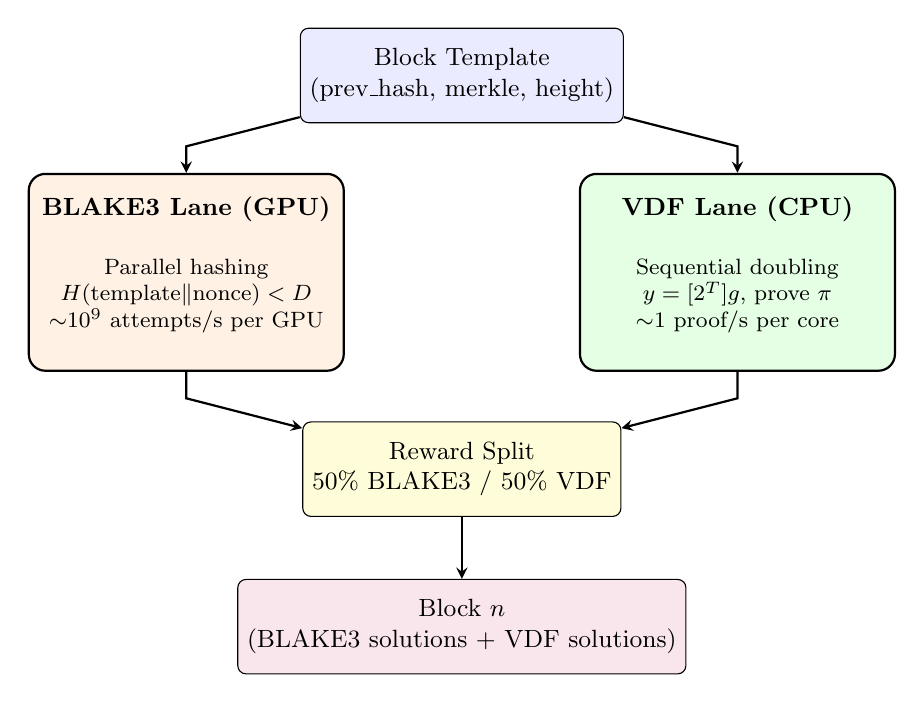
\begin{tikzpicture}[
    box/.style={draw, rectangle, rounded corners=3pt, minimum width=3.2cm, minimum height=1.2cm, align=center, font=\small},
    lane/.style={draw, rectangle, rounded corners=6pt, minimum width=4cm, minimum height=2.5cm, align=center, thick},
    arr/.style={->, thick, >=stealth}
]
    % Block template
    \node[box, fill=blue!8] (template) at (0,4.5) {Block Template\\(prev\_hash, merkle, height)};

    % BLAKE3 lane
    \node[lane, fill=orange!10] (blake3) at (-3.5,2) {};
    \node[font=\small\bfseries] at (-3.5,2.8) {BLAKE3 Lane (GPU)};
    \node[font=\footnotesize, align=center] at (-3.5,1.7) {Parallel hashing\\$H(\mathrm{template} \| \mathrm{nonce}) < D$\\$\sim$10$^9$ attempts/s per GPU};

    % VDF lane
    \node[lane, fill=green!10] (vdf) at (3.5,2) {};
    \node[font=\small\bfseries] at (3.5,2.8) {VDF Lane (CPU)};
    \node[font=\footnotesize, align=center] at (3.5,1.7) {Sequential doubling\\$y = [2^T]g$, prove $\pi$\\$\sim$1 proof/s per core};

    % Reward split
    \node[box, fill=yellow!15] (split) at (0,-0.5) {Reward Split\\50\% BLAKE3 / 50\% VDF};

    % Block
    \node[box, fill=purple!10] (block) at (0,-2.5) {Block $n$\\(BLAKE3 solutions + VDF solutions)};

    % Arrows
    \draw[arr] (template) -- (-3.5,3.6) -- (blake3);
    \draw[arr] (template) -- (3.5,3.6) -- (vdf);
    \draw[arr] (blake3) -- (-3.5,0.4) -- (split);
    \draw[arr] (vdf) -- (3.5,0.4) -- (split);
    \draw[arr] (split) -- (block);
\end{tikzpicture}
\end{center}

\subsection{Lane Specifications}

\begin{table}[h]
\centering
\begin{tabular}{lll}
\toprule
\textbf{Property} & \textbf{BLAKE3 Lane} & \textbf{VDF Lane} \\
\midrule
Hash function & BLAKE3 & Genus-2 Jacobian doubling \\
Parallelizability & Fully parallel & Strictly sequential \\
Optimal hardware & GPU (CUDA/OpenCL) & CPU (any single core) \\
GPU advantage & $>$1000$\times$ & $<$1.1$\times$ \\
Difficulty metric & Leading zero bits in hash & Fixed $T = 4{,}300$ iterations \\
Proof type & Hash preimage (32 bytes) & Wesolowski $(\pi, c)$ (145 bytes) \\
Verification cost & $O(1)$ hash evaluation & $O(\log T)$ group operations ($\sim$50 ms) \\
Reward share & 50\% of miner rewards & 50\% of miner rewards \\
\bottomrule
\end{tabular}
\caption{Comparison of the two mining lanes.}
\label{tab:lanes}
\end{table}

\subsection{Reward Distribution}

Let $R_{\mathrm{total}}$ be the total block reward and $R_{\mathrm{dev}} = 0.02 \cdot R_{\mathrm{total}}$ be the development fee. The miner reward pool is:
\begin{equation}
    R_{\mathrm{miner}} = R_{\mathrm{total}} - R_{\mathrm{dev}}
\end{equation}

After activation, the miner pool is split:
\begin{align}
    R_{\mathrm{VDF}} &= \left\lfloor R_{\mathrm{miner}} \cdot \frac{5{,}000}{10{,}000} \right\rfloor \\
    R_{\mathrm{BLAKE3}} &= R_{\mathrm{miner}} - R_{\mathrm{VDF}}
\end{align}

\begin{proposition}[Conservation]
$R_{\mathrm{BLAKE3}} + R_{\mathrm{VDF}} = R_{\mathrm{miner}}$ exactly. No rounding leak occurs between lanes because $R_{\mathrm{BLAKE3}}$ is defined as the remainder after subtracting $R_{\mathrm{VDF}}$.
\end{proposition}

Within each lane, rewards are distributed proportional to difficulty weight using division-first integer arithmetic to prevent \texttt{u128} overflow:
\begin{equation}
    r_i = \left\lfloor \frac{R_{\mathrm{lane}}}{W} \right\rfloor \cdot w_i + \left\lfloor \frac{(R_{\mathrm{lane}} \bmod W) \cdot w_i}{W} \right\rfloor
\end{equation}
where $w_i = 2^{\mathrm{leading\_zeros}(h_i)}$ is the difficulty weight of solution $i$ and $W = \sum_i w_i$. The integer rounding remainder is assigned to the highest-weight miner (deterministic tie-breaking).

\subsection{Grace Period}

To allow the VDF mining ecosystem to bootstrap, a 100-block grace period follows activation:

\begin{itemize}
    \item \textbf{Blocks 0--99 after activation:} If no VDF solutions are present, 100\% of $R_{\mathrm{miner}}$ goes to BLAKE3 miners (identical to pre-activation behavior).
    \item \textbf{Block 100+ after activation:} If no VDF solutions are present, BLAKE3 miners receive only $R_{\mathrm{BLAKE3}}$ (50\%), and the VDF allocation $R_{\mathrm{VDF}}$ is \emph{burned} (not distributed).
\end{itemize}

The burn mechanism creates a deflationary incentive for CPU miners to participate: unclaimed VDF rewards reduce total supply, benefiting all token holders.

\subsection{Height-Gated Activation}

The dual-lane split is activated at a specific block height, configurable via the \texttt{Q\_GENUS2\_VDF\_ACTIVATION\_HEIGHT} environment variable. Before this height, all solutions are treated as a single pool with the existing difficulty-weighted distribution --- ensuring \textbf{zero behavioral change} for existing miners until activation.

\begin{definition}[Activation Predicate]
\begin{equation}
    \mathrm{DualLane}(h) = \begin{cases}
        \mathsf{true} & \text{if } h \geq h_{\mathrm{activation}} \\
        \mathsf{false} & \text{otherwise}
    \end{cases}
\end{equation}
\end{definition}

This follows Quillon Graph's mainnet-safe upgrade pattern: old blocks always validate with old rules, and new rules activate automatically at the designated height without requiring node restarts.

\subsection{Determinism}

Every node must produce identical reward splits for the same block. The protocol ensures determinism through:

\begin{enumerate}
    \item \textbf{Lane classification:} A solution belongs to the VDF lane if and only if its \texttt{vdf\_output} field is \texttt{Some}. This is set during block validation and is part of the block's serialized data.
    \item \textbf{Integer-only arithmetic:} All reward calculations use \texttt{u128} integer arithmetic with no floating-point operations.
    \item \textbf{Deterministic tie-breaking:} The rounding remainder goes to the solution with the highest difficulty weight; ties are broken by index (Rust's \texttt{Iterator::max\_by\_key} returns the last maximum).
    \item \textbf{Constant share:} The VDF share is a hardcoded constant (5,000 basis points = 50\%), not a dynamic parameter.
\end{enumerate}

%% ============================================================================
\section{Security Analysis}
\label{sec:security}
%% ============================================================================

\subsection{Post-Quantum Resistance}

\begin{theorem}[Quantum Resistance of the VDF]
\label{thm:quantum}
Shor's algorithm provides no speedup for computing repeated squaring in $J(C)$.
\end{theorem}

\begin{proof}
Shor's algorithm solves the \emph{discrete logarithm problem}: given $g$ and $h = [s]g$, find $s$. The VDF problem is fundamentally different: given $g$, compute $[2^T]g$. The exponent $2^T$ is publicly known --- there is no secret to recover. The difficulty lies in the $T$ sequential group operations, each depending on the previous output. No quantum algorithm provides speedup for sequential composition of group operations. Grover's algorithm could search for a shortcut, but with a group of order $\approx 2^{512}$, Grover provides at most a $\sqrt{}$ speedup on search, which does not apply to the sequential squaring problem.
\end{proof}

\begin{theorem}[HECDLP Hardness]
The discrete logarithm problem in $J(C)$ for our genus-2 curve over a 256-bit prime field provides 128 bits of post-quantum security.
\end{theorem}

\begin{proof}
The best known classical attack on the DLP in $J(C)$ is Pollard's rho algorithm, requiring $O(\sqrt{\#J(C)}) = O(2^{256})$ group operations. The best known quantum attack is Shor's algorithm adapted for hyperelliptic curves, requiring $O(\mathrm{poly}(\log \#J(C)))$ quantum gates. For $\#J(C) \approx 2^{512}$, this provides $\lfloor 512/4 \rfloor = 128$ bits of post-quantum security against Shor's algorithm (using the standard $n/4$ heuristic for quantum security of $n$-bit DLP groups). No index calculus attack better than $O(p^{2/3})$ is known for genus-2 curves over prime fields, confirming the 128-bit security margin.
\end{proof}

\subsection{ASIC and GPU Resistance}

The VDF lane's resistance to specialized hardware stems from the sequential nature of the computation:

\begin{proposition}[Sequential Hardness]
Any hardware computing $[2^T]g$ in $J(C)$ must perform at least $T$ sequential group doublings. The critical path length is $T$, regardless of the number of parallel processing units.
\end{proposition}

\begin{proof}
Each doubling $D_{i+1} = [2]D_i$ requires $D_i$ as input. There is no known algebraic shortcut to compute $D_{i+k}$ from $D_i$ in fewer than $k$ doublings (this would require finding elements of small order in $J(C)$, which is as hard as the DLP).
\end{proof}

An ASIC or FPGA can at most reduce the \emph{latency} of a single doubling (from 200\,$\mu$s on a CPU to perhaps 120\,$\mu$s on an FPGA), but cannot increase \emph{throughput} by parallelism. This limits the maximum speedup to approximately $1.7\times$, compared to $>1{,}000\times$ for parallel hash-based mining. The economics of designing and manufacturing a VDF-specific ASIC for a $1.7\times$ advantage are unfavorable.

\subsection{Wesolowski Proof Soundness}

\begin{theorem}[Soundness]
An adversary who has not computed $T$ sequential doublings cannot produce a valid Wesolowski proof except with probability $\leq 2^{-128}$.
\end{theorem}

\begin{proof}[Sketch]
The Fiat-Shamir challenge $c$ is a 128-bit prime derived from $g$ and the claimed output $y$. To forge a proof, the adversary must find $\pi'$ such that $[c]\pi' + [r]g = y$ without knowing the correct $y$. Since $c$ is unpredictable before $y$ is committed, the adversary would need to solve the DLP in $J(C)$ to find a valid $\pi'$ for an arbitrary $c$, which requires $O(2^{128})$ work. The 128-bit challenge space ensures that random guessing succeeds with probability $\leq 2^{-128}$.
\end{proof}

\subsection{Hash-to-Curve Security}

The seed-to-element mapping uses try-and-increment with SHA3-256:

\begin{enumerate}
    \item For counter $= 0, 1, 2, \ldots$: compute $x = \mathrm{SHA3}(\texttt{"genus2-hash-to-curve-v1"} \| \mathrm{seed} \| \mathrm{counter}) \bmod p$.
    \item Evaluate $f(x) = x^5 + x^2 - 1 \bmod p$.
    \item If $f(x)$ is a quadratic residue (Euler's criterion), compute $y = \sqrt{f(x)}$ via $y = f(x)^{(p+1)/4}$ (valid since $p \equiv 3 \pmod{4}$).
    \item Return $(x, y)$ as a degree-1 divisor in $J(C)$.
\end{enumerate}

Approximately half of all $x$ values yield a quadratic residue, so the expected number of iterations is $\leq 3$. The mapping is deterministic and collision-resistant (inheriting from SHA3-256).

%% ============================================================================
\section{Implementation}
\label{sec:implementation}
%% ============================================================================

\subsection{Crate Structure}

The VDF implementation is contained in the \texttt{q-vdf} crate within the Quillon Graph workspace:

\begin{lstlisting}[language={},frame=single,basicstyle=\ttfamily\footnotesize]
crates/q-vdf/
  src/
    genus2_cantor.rs    -- Core: field arithmetic, Jacobian ops,
                           Montgomery, VDF eval, Wesolowski proofs
    lib.rs              -- Public API, VDF trait
  Cargo.toml            -- Dependencies: num-bigint, sha3, anyhow
\end{lstlisting}

Key types and their roles:

\begin{itemize}
    \item \texttt{CurveParams} --- Defines $f(x)$ coefficients and the prime $p$. The \texttt{pq128()} constructor returns the production curve $y^2 = x^5 + x^2 - 1$ over $\mathbb{F}_{2^{256}-189}$.
    \item \texttt{JacElement} --- Mumford representation $(u_1, u_0, v_1, v_0, \mathrm{degree})$. Supports canonical serialization (129 bytes), validation ($v^2 \equiv f \pmod{u}$), and seed-based deterministic construction.
    \item \texttt{MontgomeryParams} --- Precomputed Montgomery constants $(p, R \bmod p, R^2 \bmod p, p')$ as 4-limb \texttt{u64} arrays.
    \item \texttt{MontField256} --- 256-bit field element in Montgomery form. Implements \texttt{add}, \texttt{sub}, \texttt{mul}, \texttt{neg}, \texttt{inv} (Fermat).
    \item \texttt{CurveMont} --- Curve constants precomputed in Montgomery form for zero-allocation doubling.
    \item \texttt{WesolowskiProof} --- Proof $(\pi, c)$ with 145-byte serialization.
\end{itemize}

\subsection{VDF Evaluation Path}

The \texttt{evaluate\_vdf()} function selects the optimal code path based on element degree and prime size:

\begin{enumerate}
    \item If the element is degree-2 and the prime is $\geq 200$ bits: use the \textbf{Montgomery fast path}. Convert $(u_1, u_0, v_1, v_0)$ to Montgomery form once, perform all $T$ doublings via \texttt{double\_mont()}, then convert back.
    \item Otherwise: use the \textbf{BigInt fallback path} via \texttt{double\_fast()}, which uses inline polynomial arithmetic with explicit coefficient formulas.
\end{enumerate}

The Montgomery path eliminates all heap allocation in the hot loop. Each iteration of \texttt{double\_mont()} operates entirely on stack-allocated \texttt{MontField256} values (4 $\times$ \texttt{u64} each = 32 bytes per field element).

\subsection{Miner Binary}

The \texttt{q-miner} binary is an all-in-one mining client that supports both lanes:

\begin{lstlisting}[language={},frame=single,basicstyle=\ttfamily\footnotesize]
q-miner --address <WALLET> --server https://quillon.xyz
         --mode all-in-one          # Both lanes simultaneously
         --blake3-threads 0         # Auto-detect (= CPU cores)
         --vdf-threads 1            # One VDF chain per core
         --vdf-iterations 4300      # T parameter
\end{lstlisting}

In \texttt{all-in-one} mode, the miner runs BLAKE3 hashing on all available CPU threads (or a dedicated GPU via OpenCL) while simultaneously running one VDF evaluation chain per configured VDF thread. Solutions from both lanes are submitted to the server via HTTP POST.

\subsection{Server-Side Verification}

When the block producer receives a VDF solution, it verifies:

\begin{enumerate}
    \item \textbf{Challenge correctness:} The seed $g$ is derived from the block template (previous hash, merkle root, miner address) using the same deterministic hash-to-curve function.
    \item \textbf{Wesolowski proof:} $[c]\pi + [r]g = y$ (Equation~\ref{eq:verify}).
    \item \textbf{Iteration count:} The solution claims $T$ iterations; the server verifies using the same $T$.
    \item \textbf{Element validity:} Both $g$ and $y$ satisfy the Mumford conditions ($v^2 \equiv f \pmod{u}$).
\end{enumerate}

Verification takes approximately 50\,ms, which is negligible compared to the block interval.

%% ============================================================================
\section{Conclusion}
\label{sec:conclusion}
%% ============================================================================

We have presented a dual-lane mining protocol that addresses the GPU centralization problem by combining parallel BLAKE3 proof-of-work with a sequential genus-2 Jacobian VDF. The key results are:

\begin{enumerate}
    \item \textbf{CPU miners restored:} The 50/50 reward split guarantees that half of all block rewards are accessible to CPU miners, regardless of GPU hashrate on the network. A single CPU core can produce approximately one VDF proof per second, making mining economically viable on commodity hardware.

    \item \textbf{Post-quantum security:} The VDF construction based on repeated squaring in $J(C)$ for a genus-2 hyperelliptic curve provides 128-bit post-quantum security. The sequential nature of the computation renders Shor's algorithm inapplicable.

    \item \textbf{Practical performance:} Through Montgomery arithmetic with CIOS multiplication and inline polynomial composition, we achieve 200\,$\mu$s per Jacobian doubling --- an 8$\times$ improvement over the initial implementation. The complete VDF pipeline (evaluation + proof generation) completes in approximately 1 second.

    \item \textbf{Compact proofs:} Wesolowski proofs are 145 bytes regardless of the iteration count $T$, with verification in approximately 50\,ms ($O(\log T)$ group operations).

    \item \textbf{Safe deployment:} Height-gated activation, a 100-block grace period, and the burn mechanism for unclaimed VDF rewards enable a smooth transition without disrupting existing BLAKE3 miners.

    \item \textbf{Network decentralization:} By making CPU mining profitable, the dual-lane protocol increases the number of economically rational miners, reducing the Nakamoto coefficient and improving censorship resistance.
\end{enumerate}

Future work includes FPGA-targeted doubling optimizations, formal verification of the Montgomery multiplier, integration with quantum random number generators (QRNG) for VDF seed entropy, and exploration of genus-3 curves for higher security margins.

%% ============================================================================
%% APPENDICES
%% ============================================================================

\appendix

\section{Curve Parameters}
\label{app:params}

\subsection{PQ-128 Security Level (Production)}

\begin{align*}
    p &= 2^{256} - 189 \\
      &= \mathtt{0xFFFFFFFF\,FFFFFFFF\,FFFFFFFF\,FFFFFFFF\,FFFFFFFF\,FFFFFFFF\,FFFFFFFF\,FFFFFF43} \\
    f(x) &= x^5 + x^2 - 1 \\
    a_4 &= 0, \quad a_3 = 0, \quad a_2 = 1, \quad a_1 = 0, \quad a_0 = -1 \\
    \#J(C) &\approx p^2 \approx 2^{512}
\end{align*}

Montgomery constants for $R = 2^{256}$:
\begin{align*}
    R \bmod p &= 189 \\
    R^2 \bmod p &= 35{,}721 \\
    p' = -p^{-1} \bmod 2^{64} &\quad (\text{computed via 6-round Newton iteration})
\end{align*}

\subsection{VDF Parameters}

\begin{align*}
    T &= 4{,}300 \quad \text{(iterations per proof)} \\
    \text{Per-doubling latency} &\approx 200\,\mu\text{s (Montgomery, single core)} \\
    \text{Evaluation time} &\approx 0.86\,\text{s} \\
    \text{Proof generation} &\approx 0.15\,\text{s} \\
    \text{Proof size} &= 145\,\text{bytes} \\
    \text{Verification time} &\approx 50\,\text{ms}
\end{align*}

\section{Test Vectors}
\label{app:test}

\subsection{Field Arithmetic}

\begin{align*}
    p &= 115792089237316195423570985008687907853269984665640564039457584007913129639747 \\
    a &= 42, \quad b = 123456789987654321 \\
    a \cdot b \bmod p &= 5185185179481481482 \\
    a^{-1} \bmod p &= 88117163180622625322531798863572883174634940507538906315825634863122574773807 \\
    a \cdot a^{-1} \bmod p &= 1
\end{align*}

\subsection{VDF Pipeline}

For $T = 50$, seed $= \texttt{"bench\_vdf\_seed\_000"}$:
\begin{enumerate}
    \item $g = \mathrm{JacElement::from\_seed}(\mathrm{seed}, \mathrm{pq128})$ --- deterministic degree-1 element.
    \item $y = \mathrm{evaluate\_vdf}(g, 50, \mathrm{pq128})$ --- 50 sequential doublings.
    \item $(\pi, c) = \mathrm{generate\_proof}(g, y, 50, \mathrm{pq128})$ --- Wesolowski proof.
    \item $\mathrm{verify\_proof}(g, y, \pi, 50, \mathrm{pq128}) = \mathsf{true}$.
\end{enumerate}

%% ============================================================================
%% REFERENCES
%% ============================================================================

\begin{thebibliography}{12}

\bibitem{shor1994}
P.~W.~Shor, ``Algorithms for Quantum Computation: Discrete Logarithms and Factoring,'' in \textit{Proc.\ 35th Annual Symposium on Foundations of Computer Science (FOCS)}, pp.~124--134, IEEE, 1994.

\bibitem{wesolowski2019}
B.~Wesolowski, ``Efficient Verifiable Delay Functions,'' in \textit{Advances in Cryptology -- EUROCRYPT 2019}, Lecture Notes in Computer Science, vol.~11478, pp.~379--407, Springer, 2019.

\bibitem{boneh2018}
D.~Boneh, J.~Bonneau, B.~B\"{u}nz, and B.~Fisch, ``Verifiable Delay Functions,'' in \textit{Advances in Cryptology -- CRYPTO 2018}, Lecture Notes in Computer Science, vol.~10991, pp.~757--788, Springer, 2018.

\bibitem{cantor1987}
D.~G.~Cantor, ``Computing in the Jacobian of a Hyperelliptic Curve,'' \textit{Mathematics of Computation}, vol.~48, no.~177, pp.~95--101, 1987.

\bibitem{lange2002}
T.~Lange, ``Efficient Arithmetic on Genus 2 Hyperelliptic Curves over Finite Fields via Explicit Formulae,'' IACR ePrint Archive, Report 2002/121, 2002.

\bibitem{montgomery1985}
P.~L.~Montgomery, ``Modular Multiplication Without Trial Division,'' \textit{Mathematics of Computation}, vol.~44, no.~170, pp.~519--521, 1985.

\bibitem{pietrzak2019}
K.~Pietrzak, ``Simple Verifiable Delay Functions,'' in \textit{Innovations in Theoretical Computer Science (ITCS)}, 2019.

\bibitem{cohen2006}
H.~Cohen, G.~Frey, et al., \textit{Handbook of Elliptic and Hyperelliptic Curve Cryptography}, Chapman \& Hall/CRC, 2006.

\bibitem{gaudry2000}
P.~Gaudry, ``An Algorithm for Solving the Discrete Log Problem on Hyperelliptic Curves,'' in \textit{EUROCRYPT 2000}, pp.~19--34, 2000.

\bibitem{qnk_vdf_v2}
Q-NarwhalKnight Engineering Team, ``Quantum-Resistant Mining via Genus-2 Jacobian Verifiable Delay Functions,'' Quillon Graph Technical Report, Version 2.2.0, December 2025.

\bibitem{bernstein2006}
D.~J.~Bernstein, ``Curve25519: New Diffie-Hellman Speed Records,'' in \textit{Public Key Cryptography -- PKC 2006}, pp.~207--228, 2006.

\bibitem{grover1996}
L.~K.~Grover, ``A Fast Quantum Mechanical Algorithm for Database Search,'' in \textit{Proc.\ 28th Annual ACM Symposium on Theory of Computing (STOC)}, pp.~212--219, 1996.

\end{thebibliography}

\end{document}
